% !TEX root = ../thesis.tex
% [H] means put the figure HERE, directly when you input this code.
% Remove this to let LaTeX place the figure where it decides is best
\begin{figure}[H]
	\centering
	
% We use a figure width of 48.5% of the width of one line of text on 
% the page so there is some space between the images.
	\subfloat[Image 1]{
		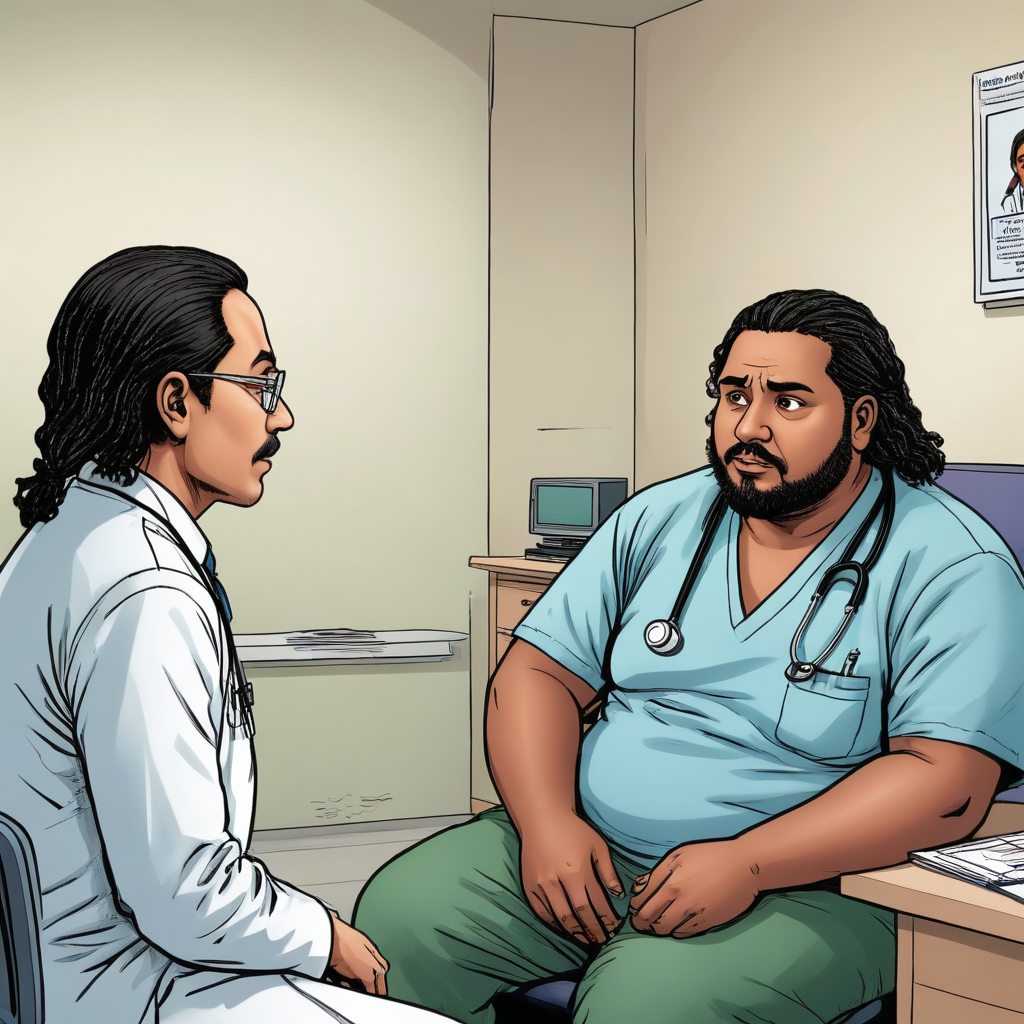
\includegraphics[width=0.235\textwidth]{graphics/consistency (1).png}\label{fig:example_2x2_a}
	}
	\hfill % Spacing between sub-figures displayed next to each other.
	\subfloat[Image 2]{
		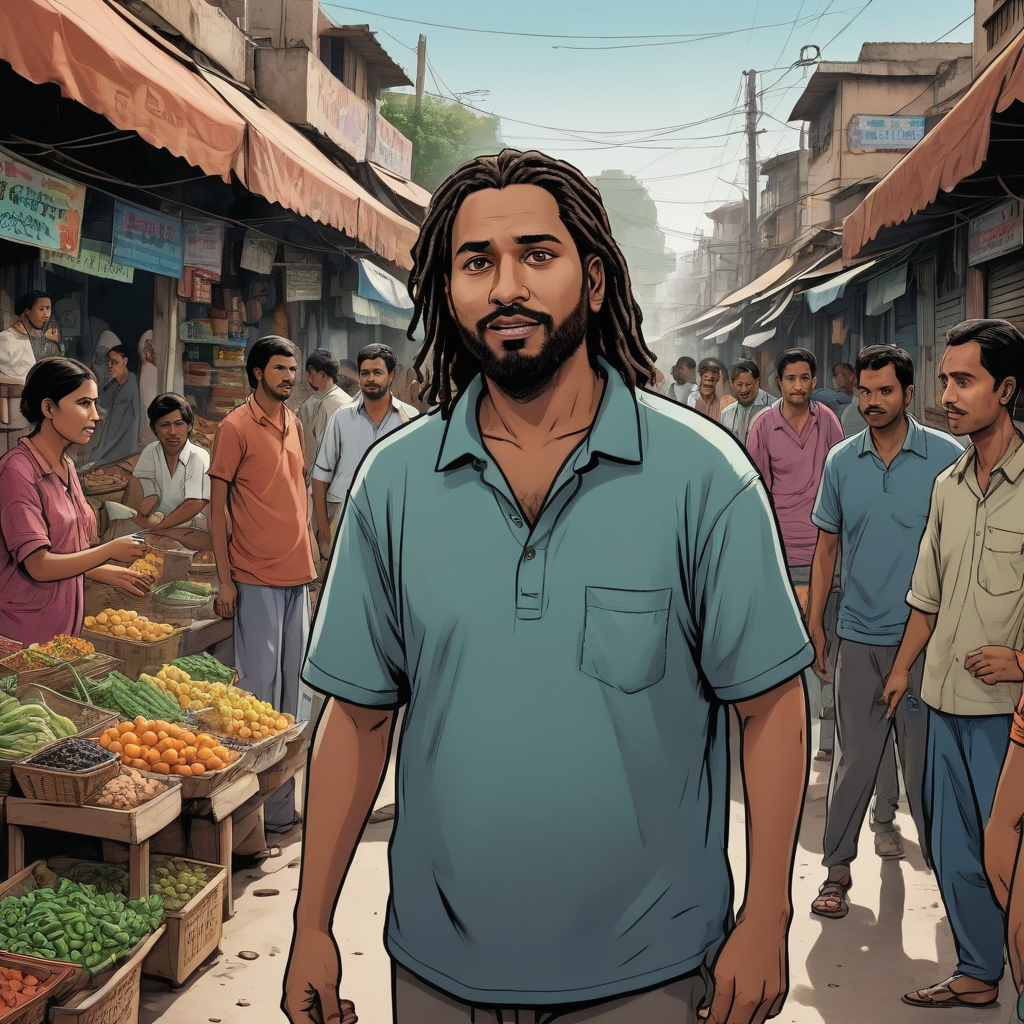
\includegraphics[width=0.235\textwidth]{graphics/consistency (2).png}\label{fig:example_2x2_b}
	}
	% \\ % New line before caption.
	\hfill % Spacing between sub-figures displayed next to each other.
	\subfloat[Image 3]{
		
\includegraphics[width=0.235\textwidth]{graphics/consistency (3).png}\label{fig:example_2x2_c}
	}
	\hfill % Spacing between sub-figures displayed next to each other.
	\subfloat[Image 4]{
		
\includegraphics[width=0.235\textwidth]{graphics/consistency (4).png}\label{fig:example_2x2_d}
	}
	\\ % New line before caption.
		
% Caption is defined with a short and long version. The short version is shown in the 
% List of Figures section, and the long version is used directly with the figure. 	
	\caption[All images depict the same patient looking different]{
All images depict the same patient looking different.
	
% Figure labels should be defined at the end of the caption to ensure proper numbering.
	\label{fig:consistency}
	}
	
\end{figure}